\chapter{Investigating the sub-continental ancestry of ethnic minorities within the UK Biobank from sparse genotype data}
\label{chapterlabel3}

\section{Introduction}

From a genetic standpoint, the native British population is one of the most highly studied in the world \cite{Leslie2015, }.


Despite this, the roughly 8 million ethnic minorities within the U.K. remain relatively understudied. For example, all of the 27 papers were deposited between  in the GWAS catalogue “UK Biobank” in the title between 



We took advantage of the U.K. Biobank (UKB) resource and detailed reference panel of worldwide individuals (Human Origins) in order to investigate the ancestry of the ethnic minorities within the UKB. 

\section{Methods}

\subsection{Data access}

Access was obtained to study the UK Biobank dataset via UCL genetics institute. 

\subsection{ADMIXTURE analysis}

Performing chromopainter analysis on the entire UK Biobank dataset (n=488,377 individuals) is currently computationally infeasible. Thus, we chose to analyse only a subset of individuals; a) individuals with more than 50\% non-European ancestry, b) individuals who had recieved a Covid-19 test.

To identify individuals who had more than 50\% non-European ancestry, we split all UK Biobank individuals into 100 batches and performed supervised ADMIXTURE \cite{alexander2009fast} analysis on each batch. Prior to performing ADMIXTURE, we LD pruned the SNPs using the plink \cite{purcell2007plink} command --indep-pairwise 50 10 0.02, retaining 70,776 SNPs. The pruned UK Biobank dataset was then merged with the 1000 genomes genotypes \cite{10002010map}. 

I ran a supervised ADMIXTURE analysis on each batch by using the --supervised command and fixing the 4 reference populations as GBR British, Nigeria Yoruba, Han Chinese and Gujarati Indian. The rest of the arguments were left to default.

\subsection{Data preparation - imputed data}

To jointly analyse the UK Biobank the Human Origins datasets, it is necessary to merge them and retain only SNPs which have been genotyped in both datasets (i.e. contain no missing genotypes). The number of common SNPs between the UK Biobank chip and the Human Origins chip was 65,727. Using this number of SNPs in the chromosome painting analysis may reduce power to detect fine-scale genetic differences between samples relative to using the roughly 500,000 SNPs present. One option is to therefore use the imputed UK Biobank dataset \cite{bycroft2018uk}. This has been imputed using the haplotype reference consortium reference panel \cite{mccarthy2016reference}.

The imputed data was downloaded and converted from .bgen to .vcf format using qctool. Strand inconsistencies between the UK Biobank and Human Origins dataset were identified using the gt-conform utilty from Beagle and any inconsistent positions removed. The Human Origins and UK Biobank datsets were then merged using the bcftools merge command. The resulting merged dataset contained 493,407 individuals and 535,544 SNPs.

The merged dataset was then phased using shapeit4 \cite{delaneau2018integrative}, setting --pbwt-depth 1 to increase speed at this large sample size. The phased output was converted to chromopainter output using a custom script.

\subsection{Data preparation - non imputed data}

I also performed an analysis using only the 65,727 SNPs which overlap exactly between the UK Biobank chip and the Human Origins chip. 

plink1.9 \cite{purcell2007plink} was used to convert the binary plink files to bgzipped vcf format. The resulting vcf was filtered to include only those common with the Human Origins SNPs using bcftools view \cite{li2009sequence} and those individuals which had either a) at least 50\% non-European ancestry or b) for which we have data on Covid-19 test, leaving 26,298 individuals. The filtered UK Biobank dataset was then merged with the Human Origins dataset using bcftools merge.

I next phased the merged UK Biobank / Human Origins dataset using shapeit4 \cite{delaneau2018integrative}. I set --pbwt-depth 8 and left all other parameters as default. The resulting vcf of phased haplotypes was converted to chromopainter format using a custom script (appendix?).  

\subsection{Imputation bias test}

When using a reference panel of individuals comprising primarily of European individuals, imputating genotypes in individuals of majority non-European ancestry can be innacurate. Therefore, we needed to test the effect of genotype imputation on the estimated copyvectors and ancestry proportions in the African UK Biobank individuals. 

To do this, we took the entire Human Origins dataset (5998 individuals and 560,420 SNPs) and submitted it to the Sanger Imputation Server, using the full Haplotype Reference Consortium (HRC) as a reference for phasing and imputation. This reference panel was chosen because it was the same one used for imputing the Biobank individuals.

I next subsetted the imputed Human Origins dataset down to SNPs present in the UK Biobank array , leaving 727,325 positions present in the imputed Human Origins dataset. I then performed an 'all-v-all' painting, forming each target haplotype as a mosaic of all other haplotypes. I also performed an identical 'all-v-all' painting of the same Human Origins dataset, but using the original set of SNPs where none had been imputed. 

Therefore, we had 2 coancestry matrices of identical struture, but one was generated using a majority of imputed SNPs and the other was generated using no imputed SNPs. 

I also performed SOURCEFIND analysis on both matrices. Individuals were grouped into populations and all populations were used as surrogates for each target population. Default parameters were used and each SOURCEFIND target was analysed for 2,000,000 MCMC iterations. Ancestry proportions and confidence intervals were estimated from the raw MCMC output using the Coda R library \cite{oro22547}.

\subsection{Chromopainter}

After the decision to not use the imputed data, we performed the following painting analysis using the dataset described above in "Data preparation - non imputed data". To maximise efficiency, we performed 2 different paintings.

Firstly, we performed an all-v-all painting of the Human Origins dataset (excluding the admixed individuals assigned to the AA Denver population). Secondly, we painted each of the retained UK Biobank individuals (n=26,298) as recipients and all non AA Denver individuals as donors. The resulting coancestry matrices for these 2 paintings were then combined with one another to give a combined coancestry matrix with Human Origins individuals as donors (n=5998) and Human Origins + retained UK Biobank individuals as recipients (n=32,296).

\subsection{SOURCEFIND}

\section{Results}

\subsection{ADMIXTURE}

I performed supervised ADMIXTURE on all 488,378 UK Biobank individuals in order to identify individuals with at least 50\% non-European ancestry. These individuals would then be carried forward to later analyses. In total, there were 8476, 2653, 9171 indivisuals with at least 50\% ancestry from Yoruba, Han Chinese and Gujarati reference populations respectively. 

To verify the accuracy of the ADMIXTURE results, I selected all individuals who self-identified as being either "Caribbean", "African" or "Black or Black British" (n=7527) and assessed the distribution of ADMIXTURE ancestry proportions, under the assumption that these individuals should contain more African than other kinds of ancestry. This was the case, with the mean proportion of African ancrstryn amongst these individuals being 0.85 (Fig. \cite{African_Inds_proportions_ADMIXTURE}.

We observed substantial variation in the ancestry proportions for those self-identified as being either "Caribbean", "African" or "Black or Black British" - proportions of Yoruban and British ancestry ranged from 0.00001 to 1, Han Chinese from 0.00001 to 0.53 and Gujarati from 0.759 to 0.00001, reflecting the diverse array of genetic ancestries that can fall under a given ethnic label.


\begin{figure}[htp]
    \centering
    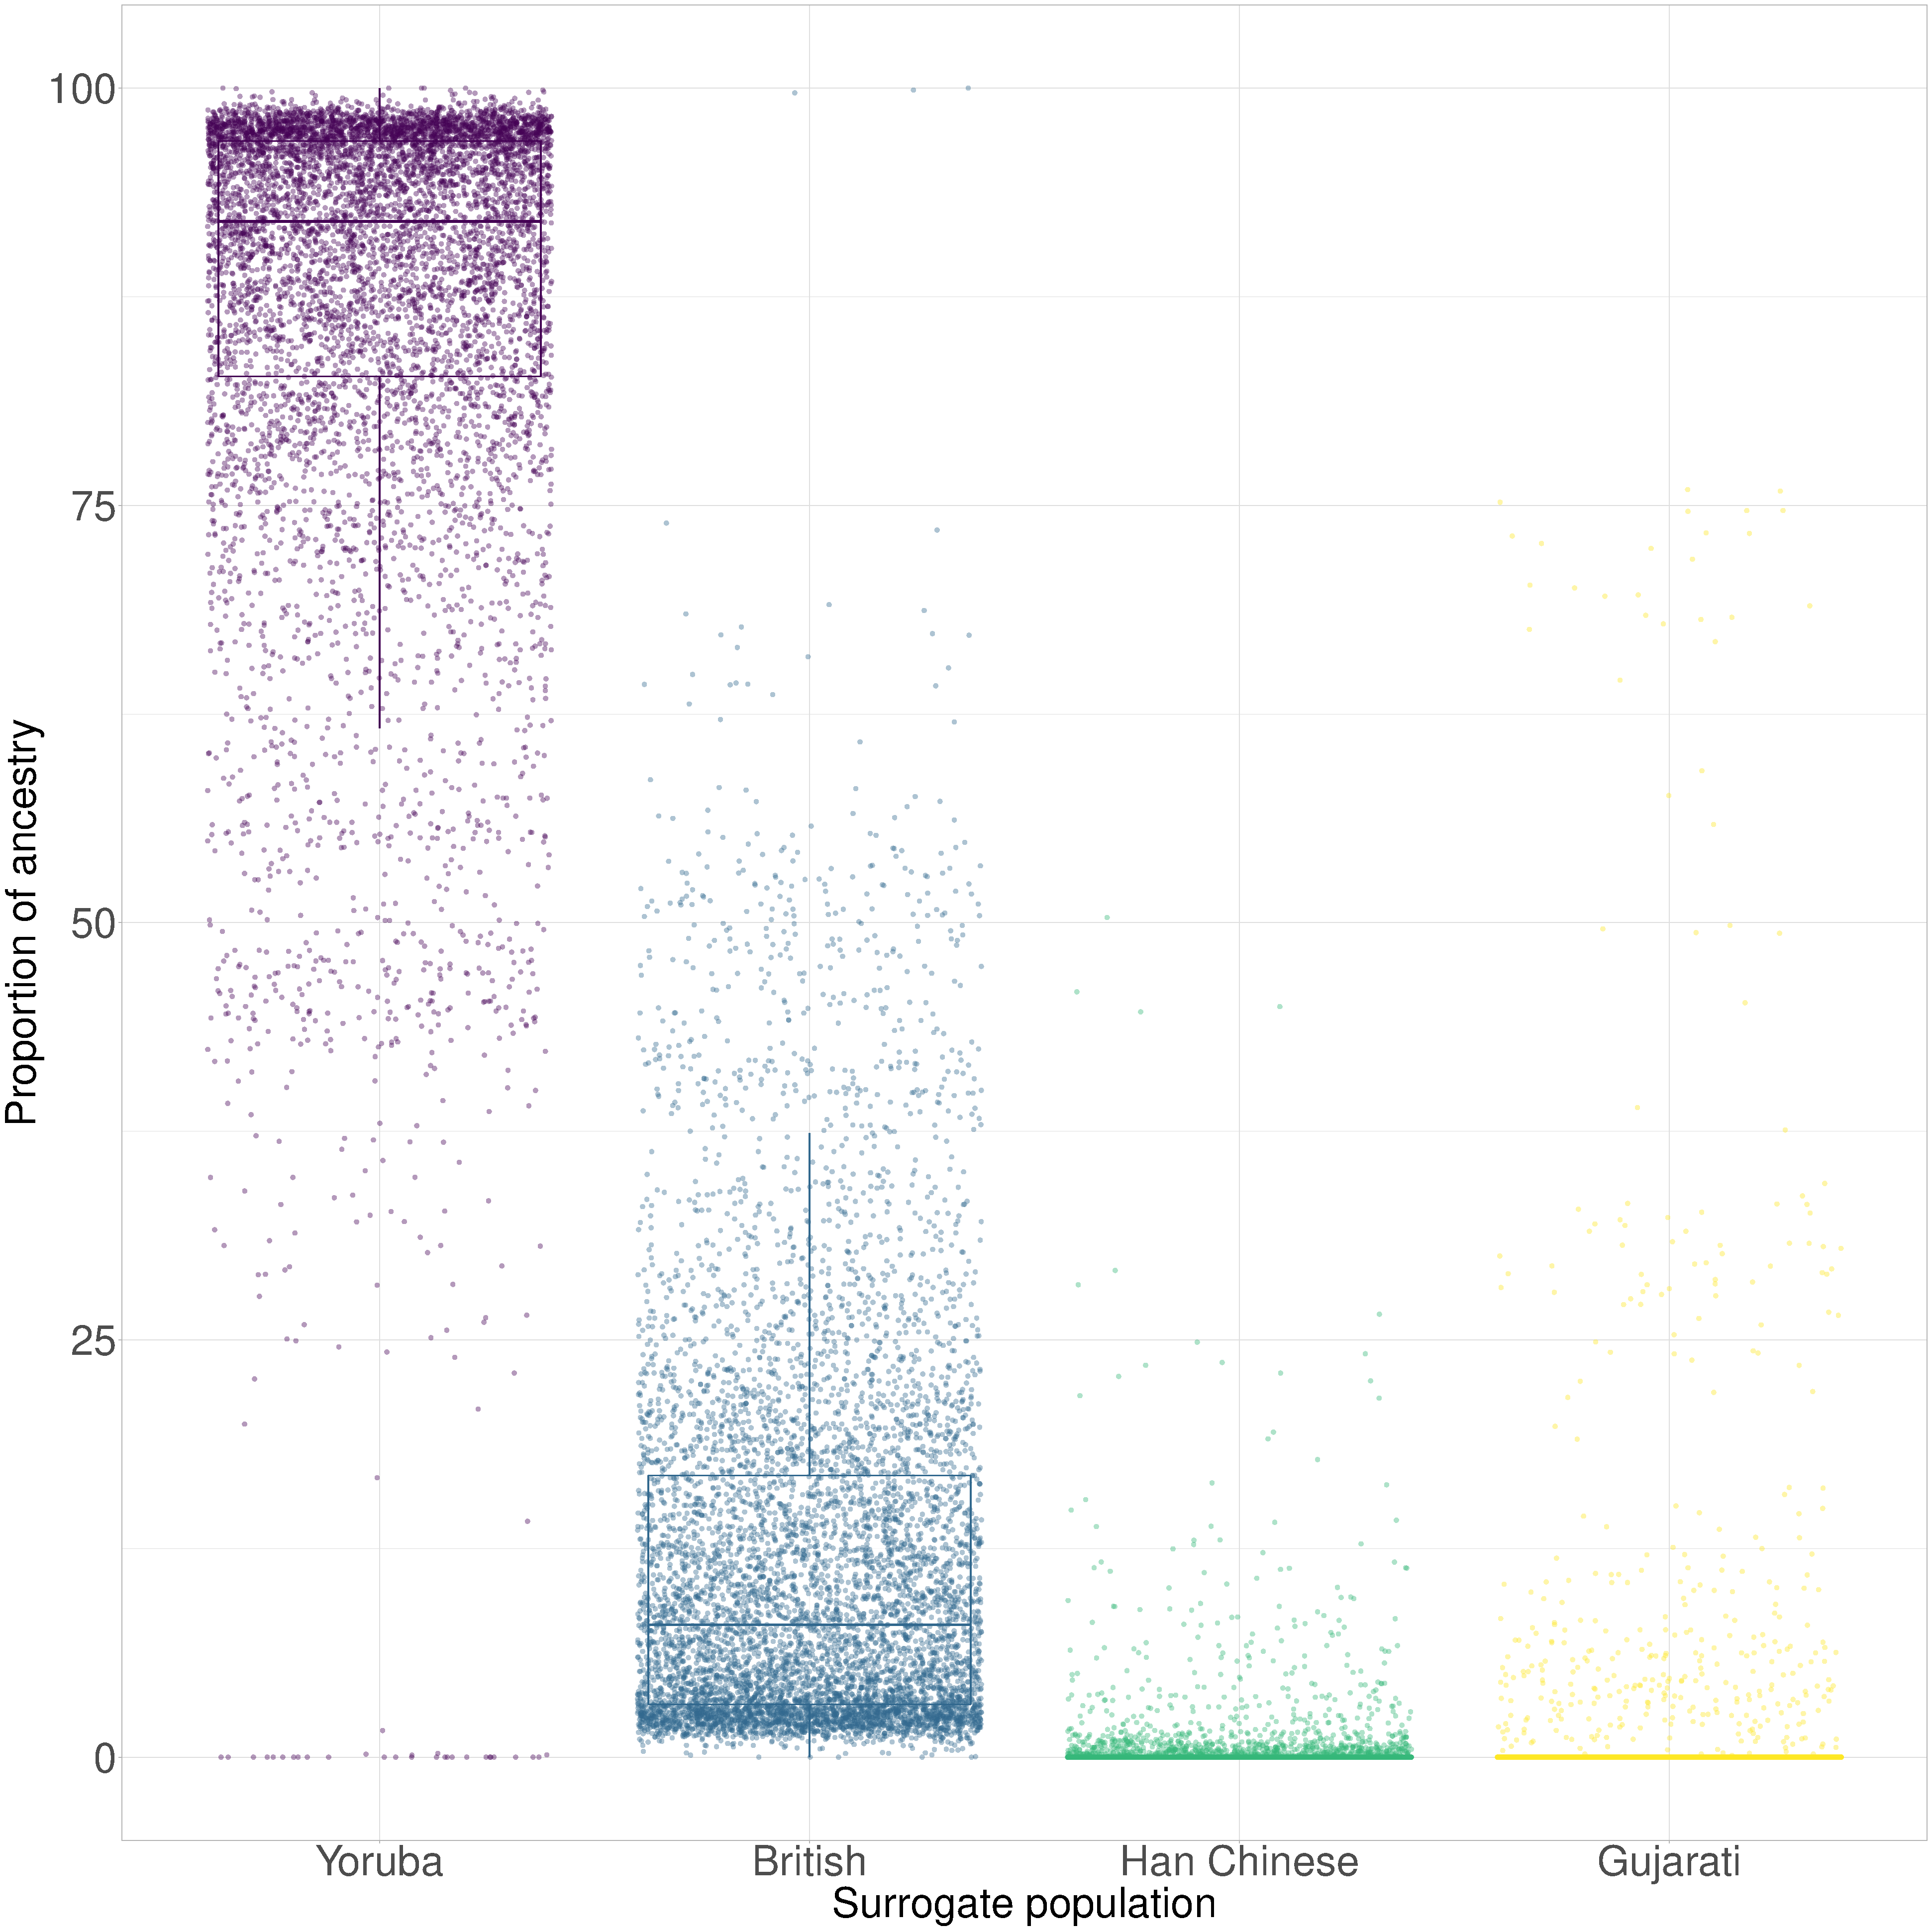
\includegraphics[width=1.0\textwidth]{../images/chapter3/African_Inds_proportions.pdf}
    \caption{Ancestry proportions inferred from supervised Admixture run (k=4) for all individuals who self identified as being either "Caribbean", "African" or "Black or Black British".}
    \label{fig:African_Inds_proportions_ADMIXTURE}
\end{figure}


\subsection{Chromopainter}

Our Chromopainter analysis generated a 27,529 x 5999 co-ancestry matrix. Principle component analysis on this matrix reveals the general structure of the selected individuals, alongside the reference populations (Fig. \ref{fig:/PCA_chunklengths_HumanOrigins_UKBiobank})

\begin{figure}[htp]
    \centering
    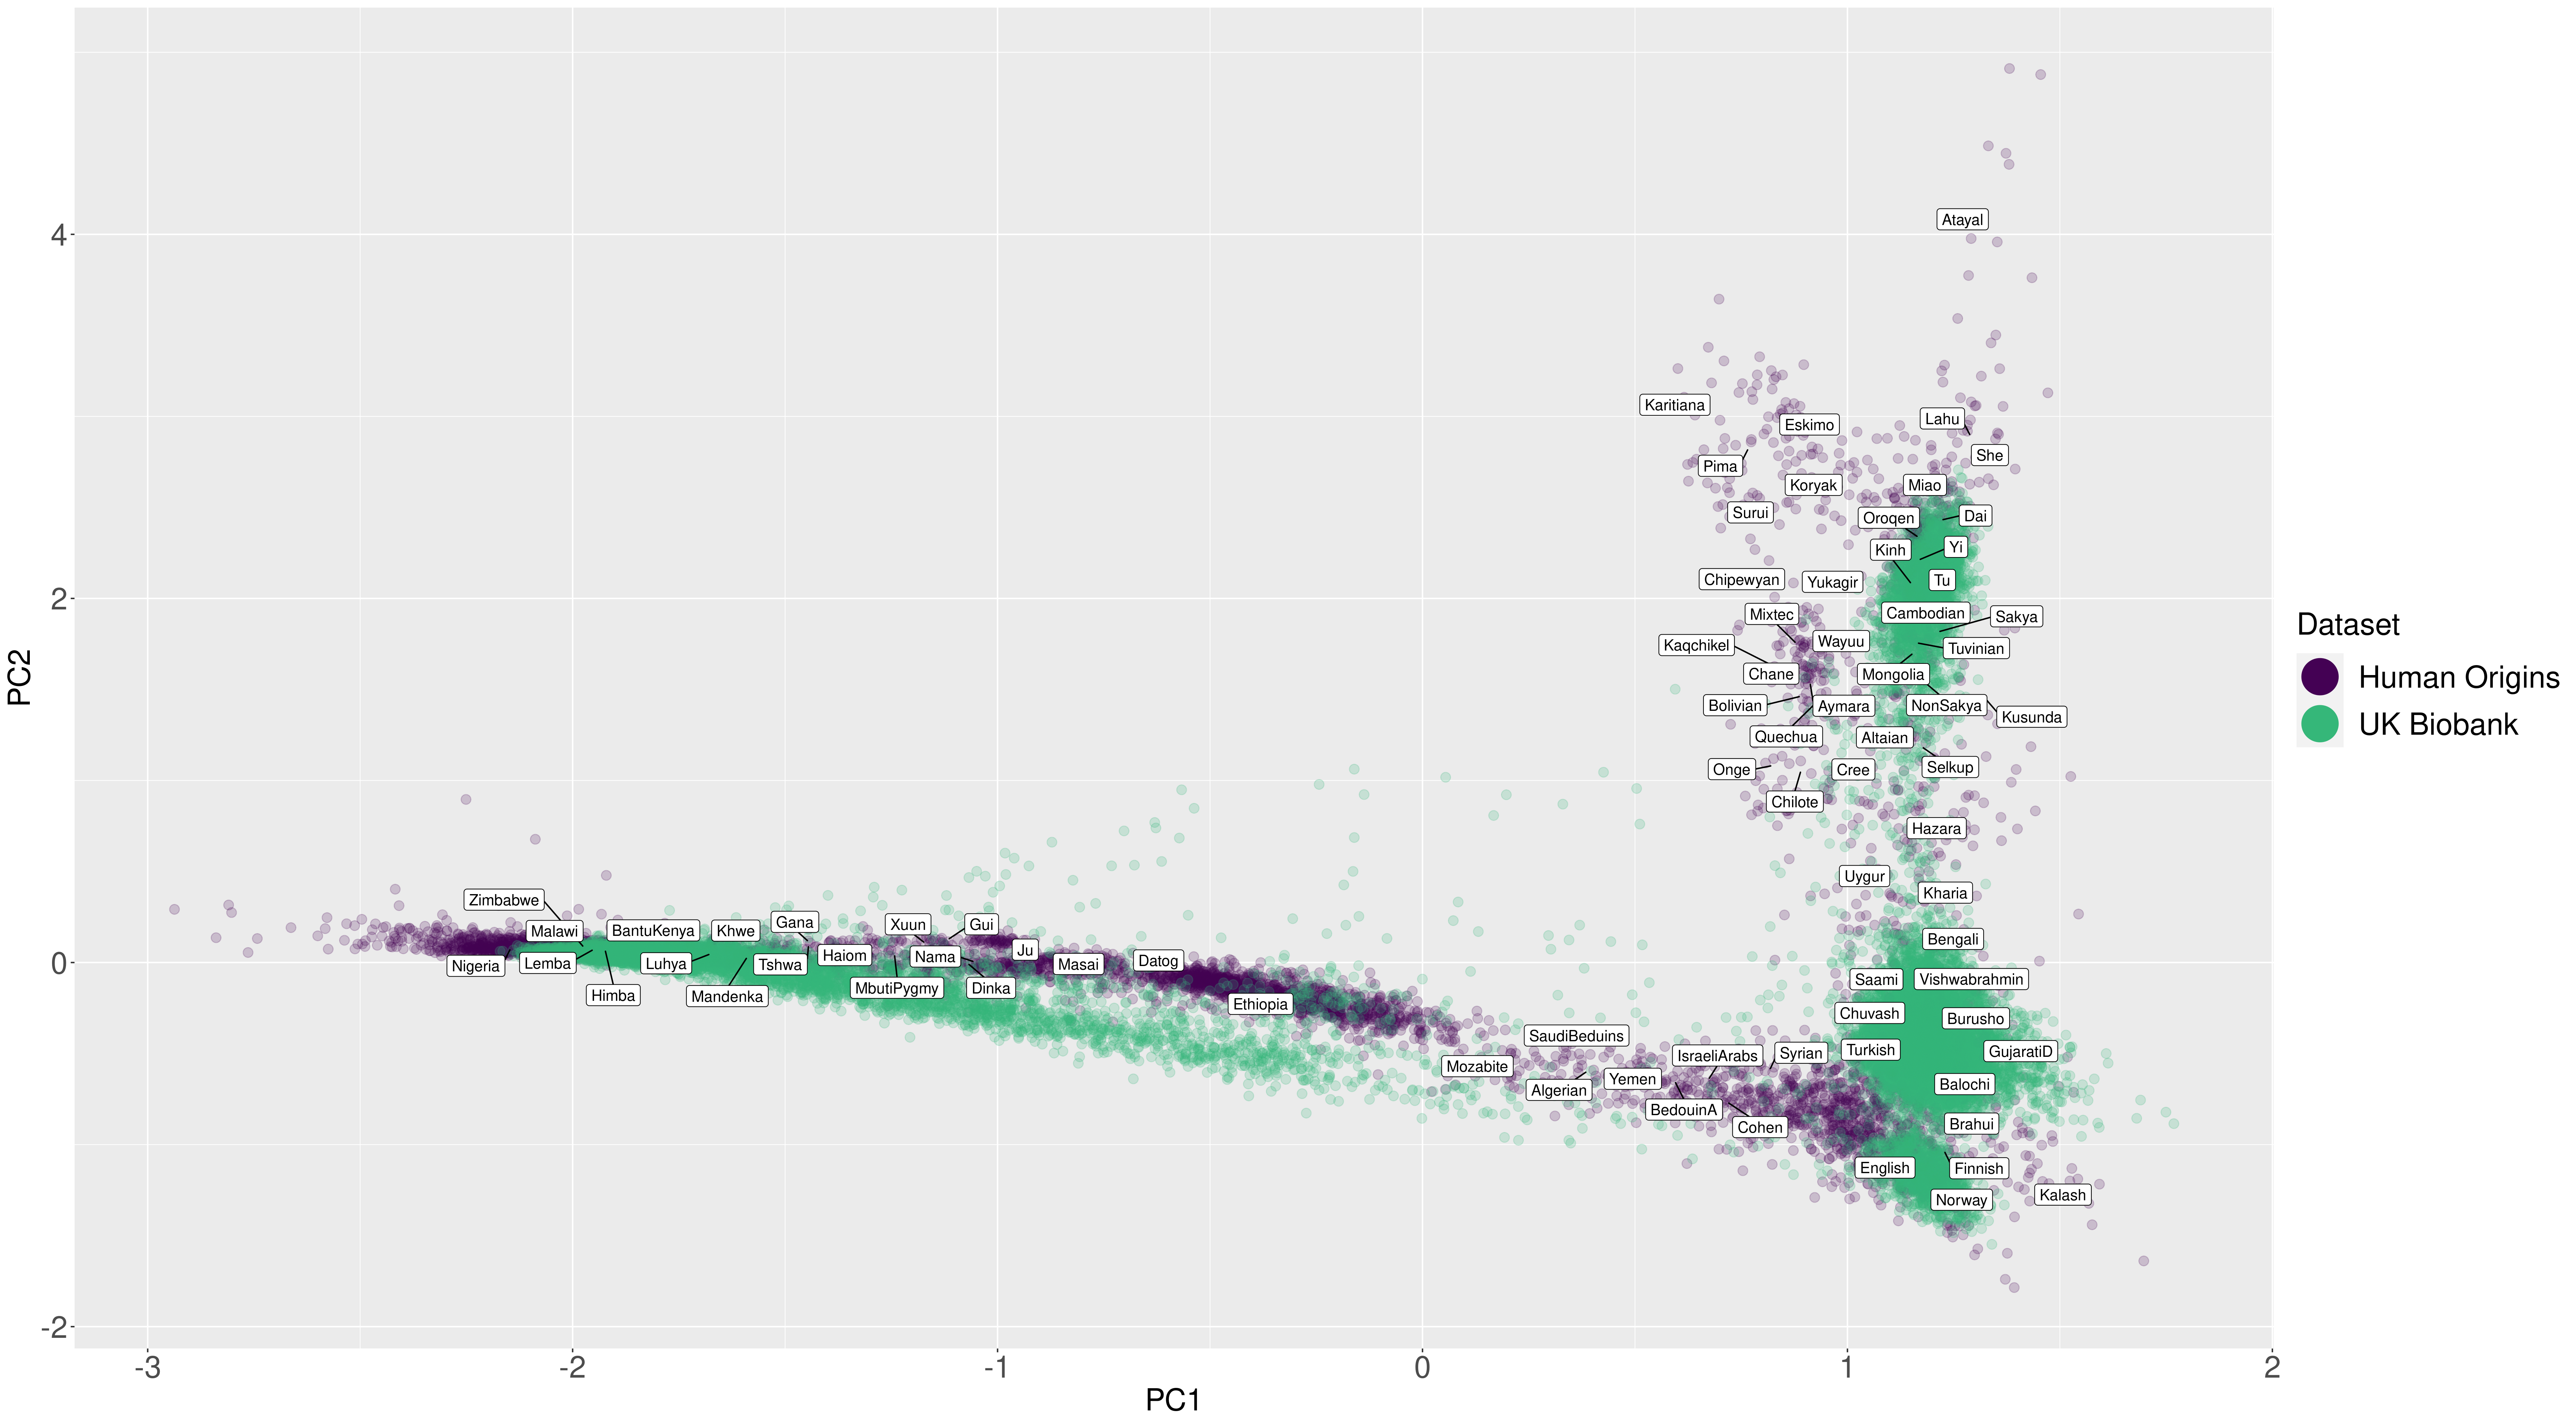
\includegraphics[width=1.0\textwidth]{../images/chapter3/PCA_chunklengths_HumanOrigins_UKBiobank.png}
    \caption{Principle component analysis of chunklengths matrix for all African UK Biobank individuals and human origins array. Individuals are coloured dependent on whether they are UK Biobank (green) or Human Origins (purple) samples. Labels indicate mean principle component coordinates for individuals in that population. A random sample of populations were chosen to have labels to prevent the figure from being too cluttered.}
    \label{fig:/PCA_chunklengths_HumanOrigins_UKBiobank}
\end{figure}

Aggregating the columns of the aforementioned co-ancestry matrix by reference population by mean/sum gives the total length of genome each UK Biobank individual most closely matches individuals from that reference population. This can be visualised on a map, where each point represents a reference population and the colour corresponds to the total amount that reference population contributes towards the ancestry of all retained UK Biobank individuals (Fig. \ref{fig:haplotype_sharing_map_zoomed_II}).

\begin{figure}[htp]
    \centering
    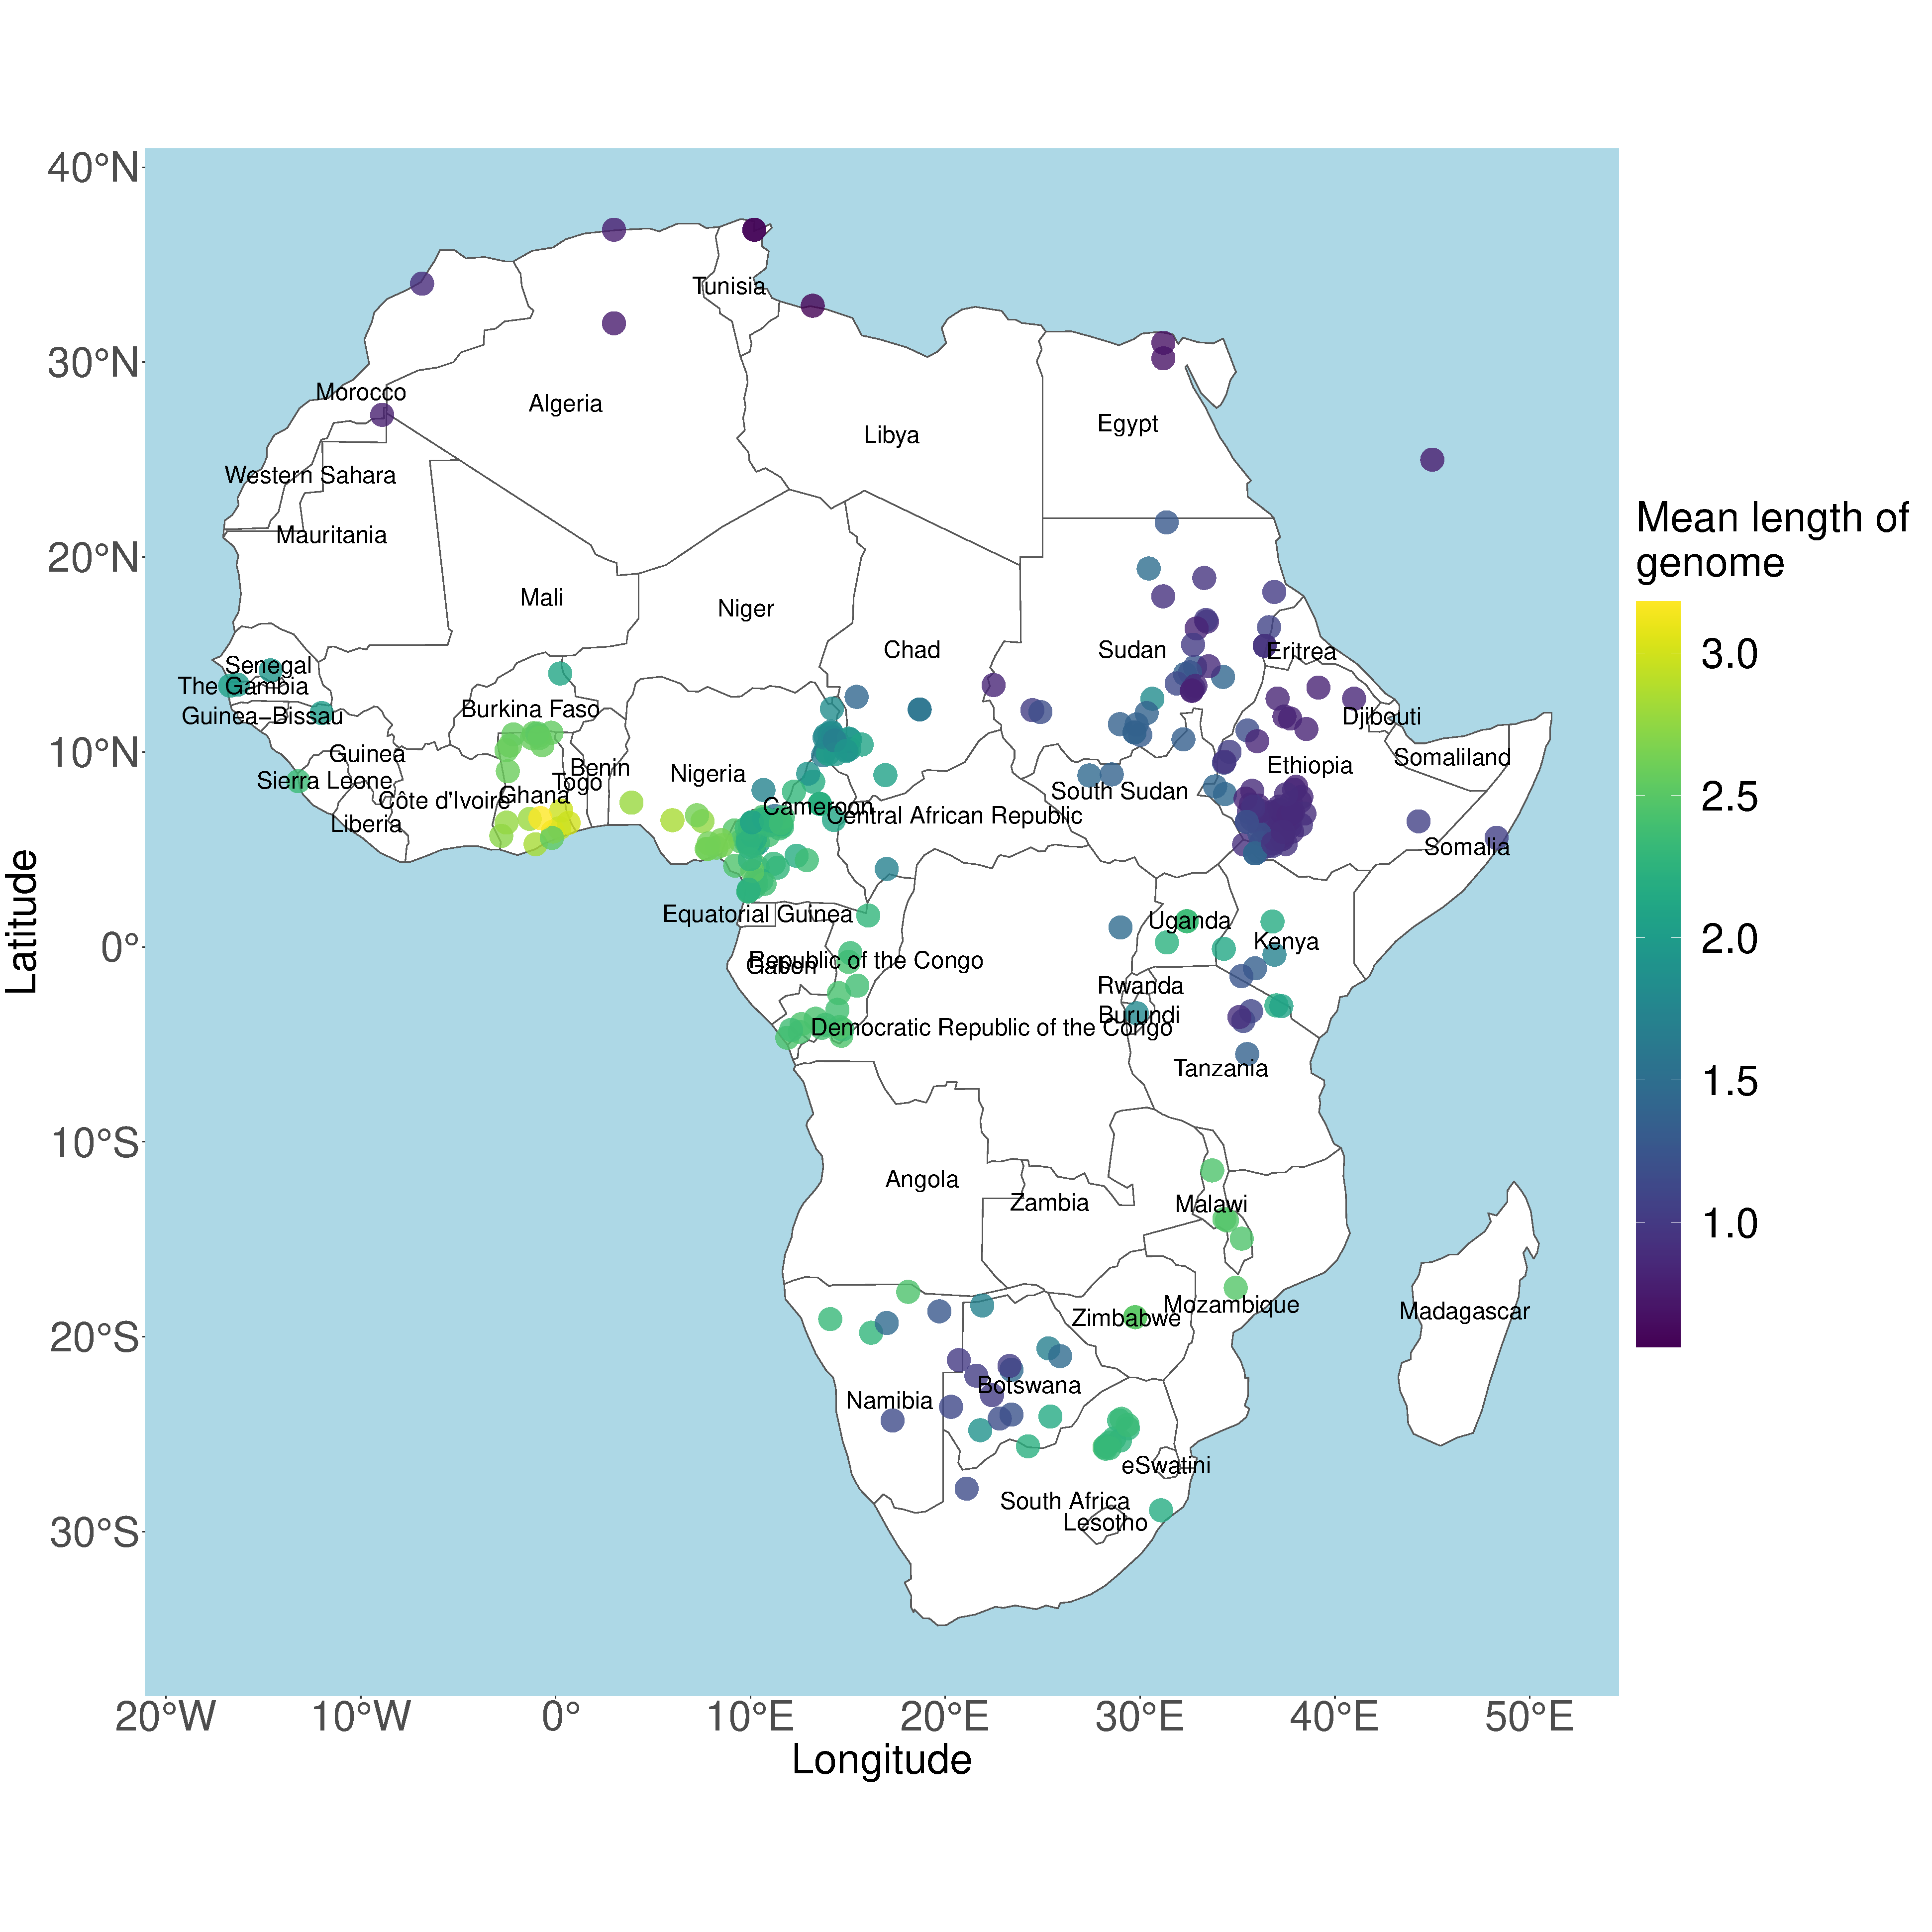
\includegraphics[width=1.0\textwidth]{../images/chapter3/haplotype_sharing_map_zoomed_II.pdf}
    \caption{Map of haplotype donation to UK Biobank individuals. Each point represents a different African population. Colour }
    \label{fig:haplotype_sharing_map_zoomed_II}
\end{figure}

The populations with the largest contribution to the retained UK Biobank samples are those from West Africa. This is consistent with two different historical processes. 

Firstly, it is known from historical and genetic studies that a majority of the individuals who were forcibly transported from Africa to the Americas during the transatlantic slave trade were from the west coast of Africa \cite{micheletti2020genetic}. Given the UK Biobank sample contains many individuals who were either born in, or trace their ancestry from the Caribbean, we would expect there to be a large contribution of ancestry from West Africa.

Secondly and more recently, there has been a relatively large amount of historical immigration from countries in West Africa, such as Ghana and Nigeria, to the U.K. 

\subsection{Verifying painting accuracy}

Given the total number of SNPs used in the analysis (n=65,727) is on an order of magnitude less than is typically used in such analysis, it is important to verify the results do not simply correspond to copying the most from the reference populations with the largest sample size, as has been shown in previous analyses (refer to previous chapters). To test that the coancestry matrix contains relevant information about the ancestry of the retained UK Biobank individuals, I took advantage of the UK Biobank metadata and subsetted the coancestry matrix to contain only individuals who were born in a particular country. We would expect that individuals who were born in a particular country would copy the most from reference populations from that country. For example, we would expect individuals who were born in South Africa to copy the most from Bantu and Zulu ethnic groups from South Africa. 

\begin{figure}[htp]
    \centering
    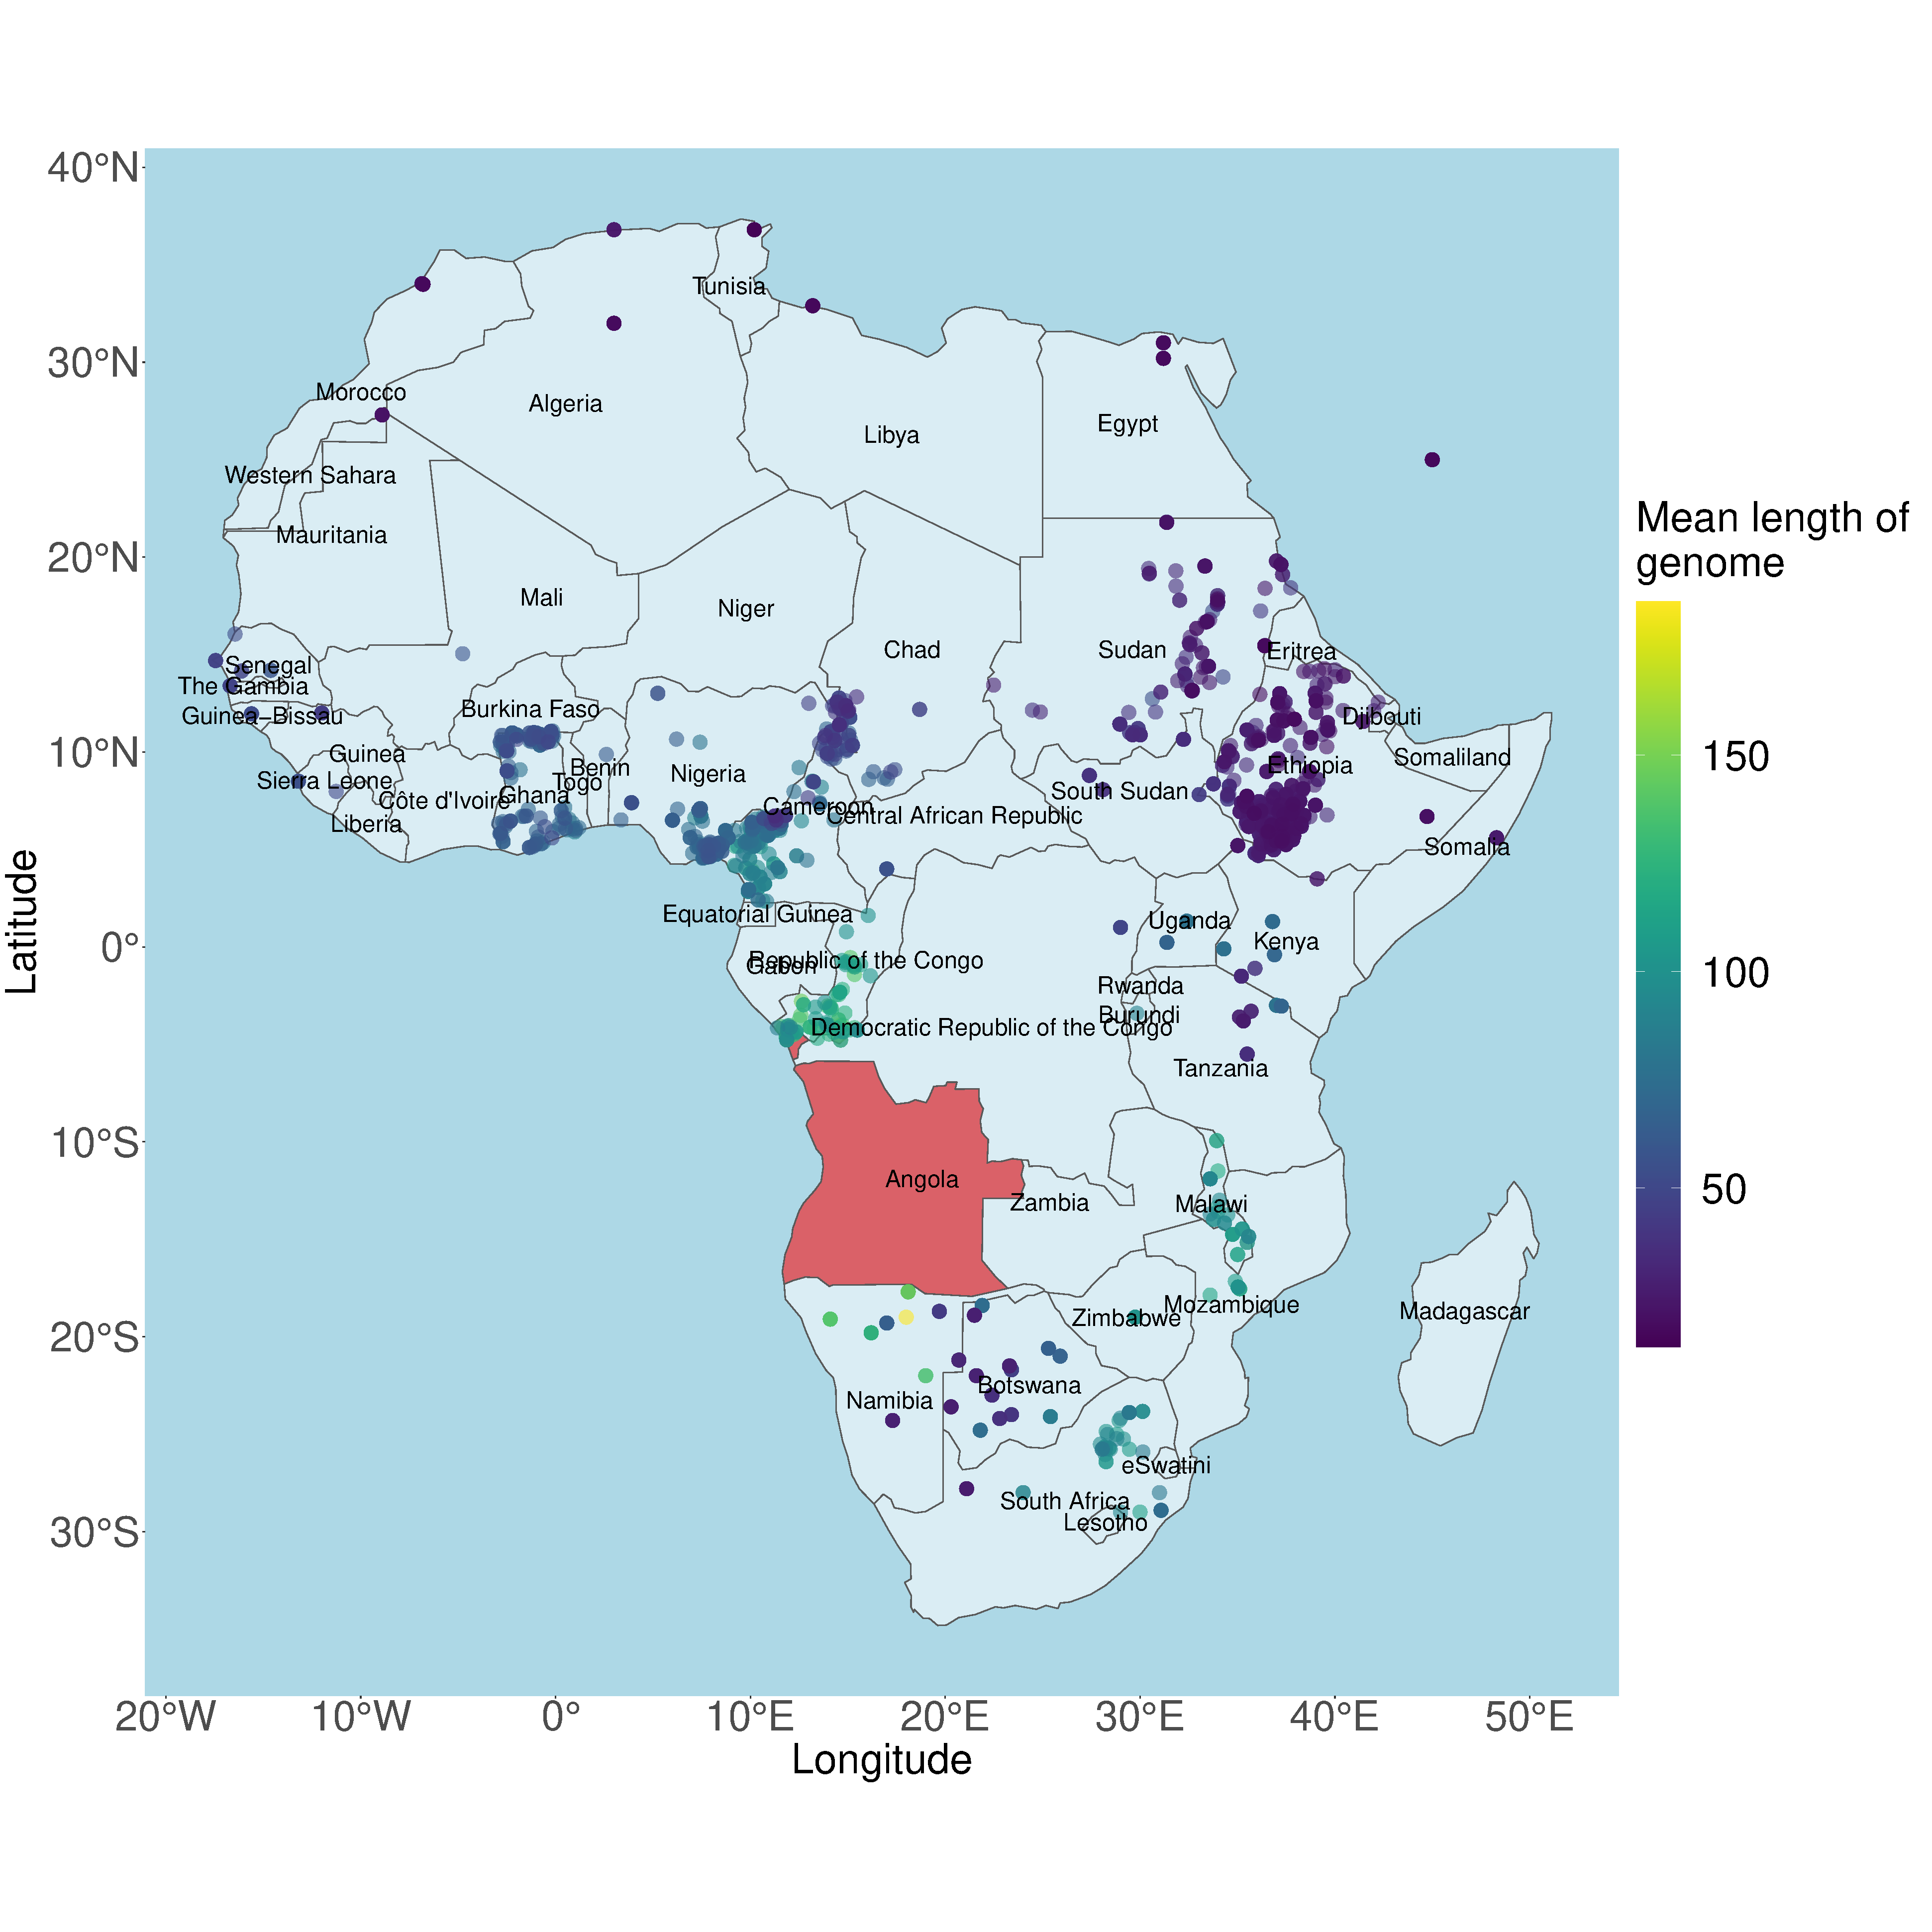
\includegraphics[width=1.0\textwidth]{../images/chapter3/haplotype_map_SouthAfrica.pdf}
    \caption{Map of haplotype donation to UK Biobank individuals born in South Africa.}
    \label{fig:haplotype_map_South Africa}
\end{figure}

Fig. \ref{fig:haplotype_map_South Africa} shows the map of haplotype donation from reference groups to UK Biobank individuals born in South Africa. It is clear that reference populations from South Africa, in particular the Zulu ethnic group, contribute the most to these individuals. The same pattern is clear for most countries of origin. 

There are several interesting cases. For example, there are N individuals who were born in the Caribbean. Visualising the haplotype donation map for these individuals shows that they are primarily of West African ancestry, consistent with historical evidence \cite{micheletti2020genetic}. Individuals born in Brazil have ancestry from further South, again consistent with historical evidence (citation needed).

As a more formal test of the painting accuracy, I estimated SOURCEFIND ancestry proportions in each retained UK Biobank individuals. An individual was 'assigned' to a particular reference population if they had 75\% or more ancestry from that population. If the country the assigned reference population is from matches the birth location of the individual, then I considered that a 'success' and a 'fail' otherwise. Individuals who were born in the U.K. or who had no birth country were excluded from this analysis. 

\begin{figure}[htp]
    \centering
    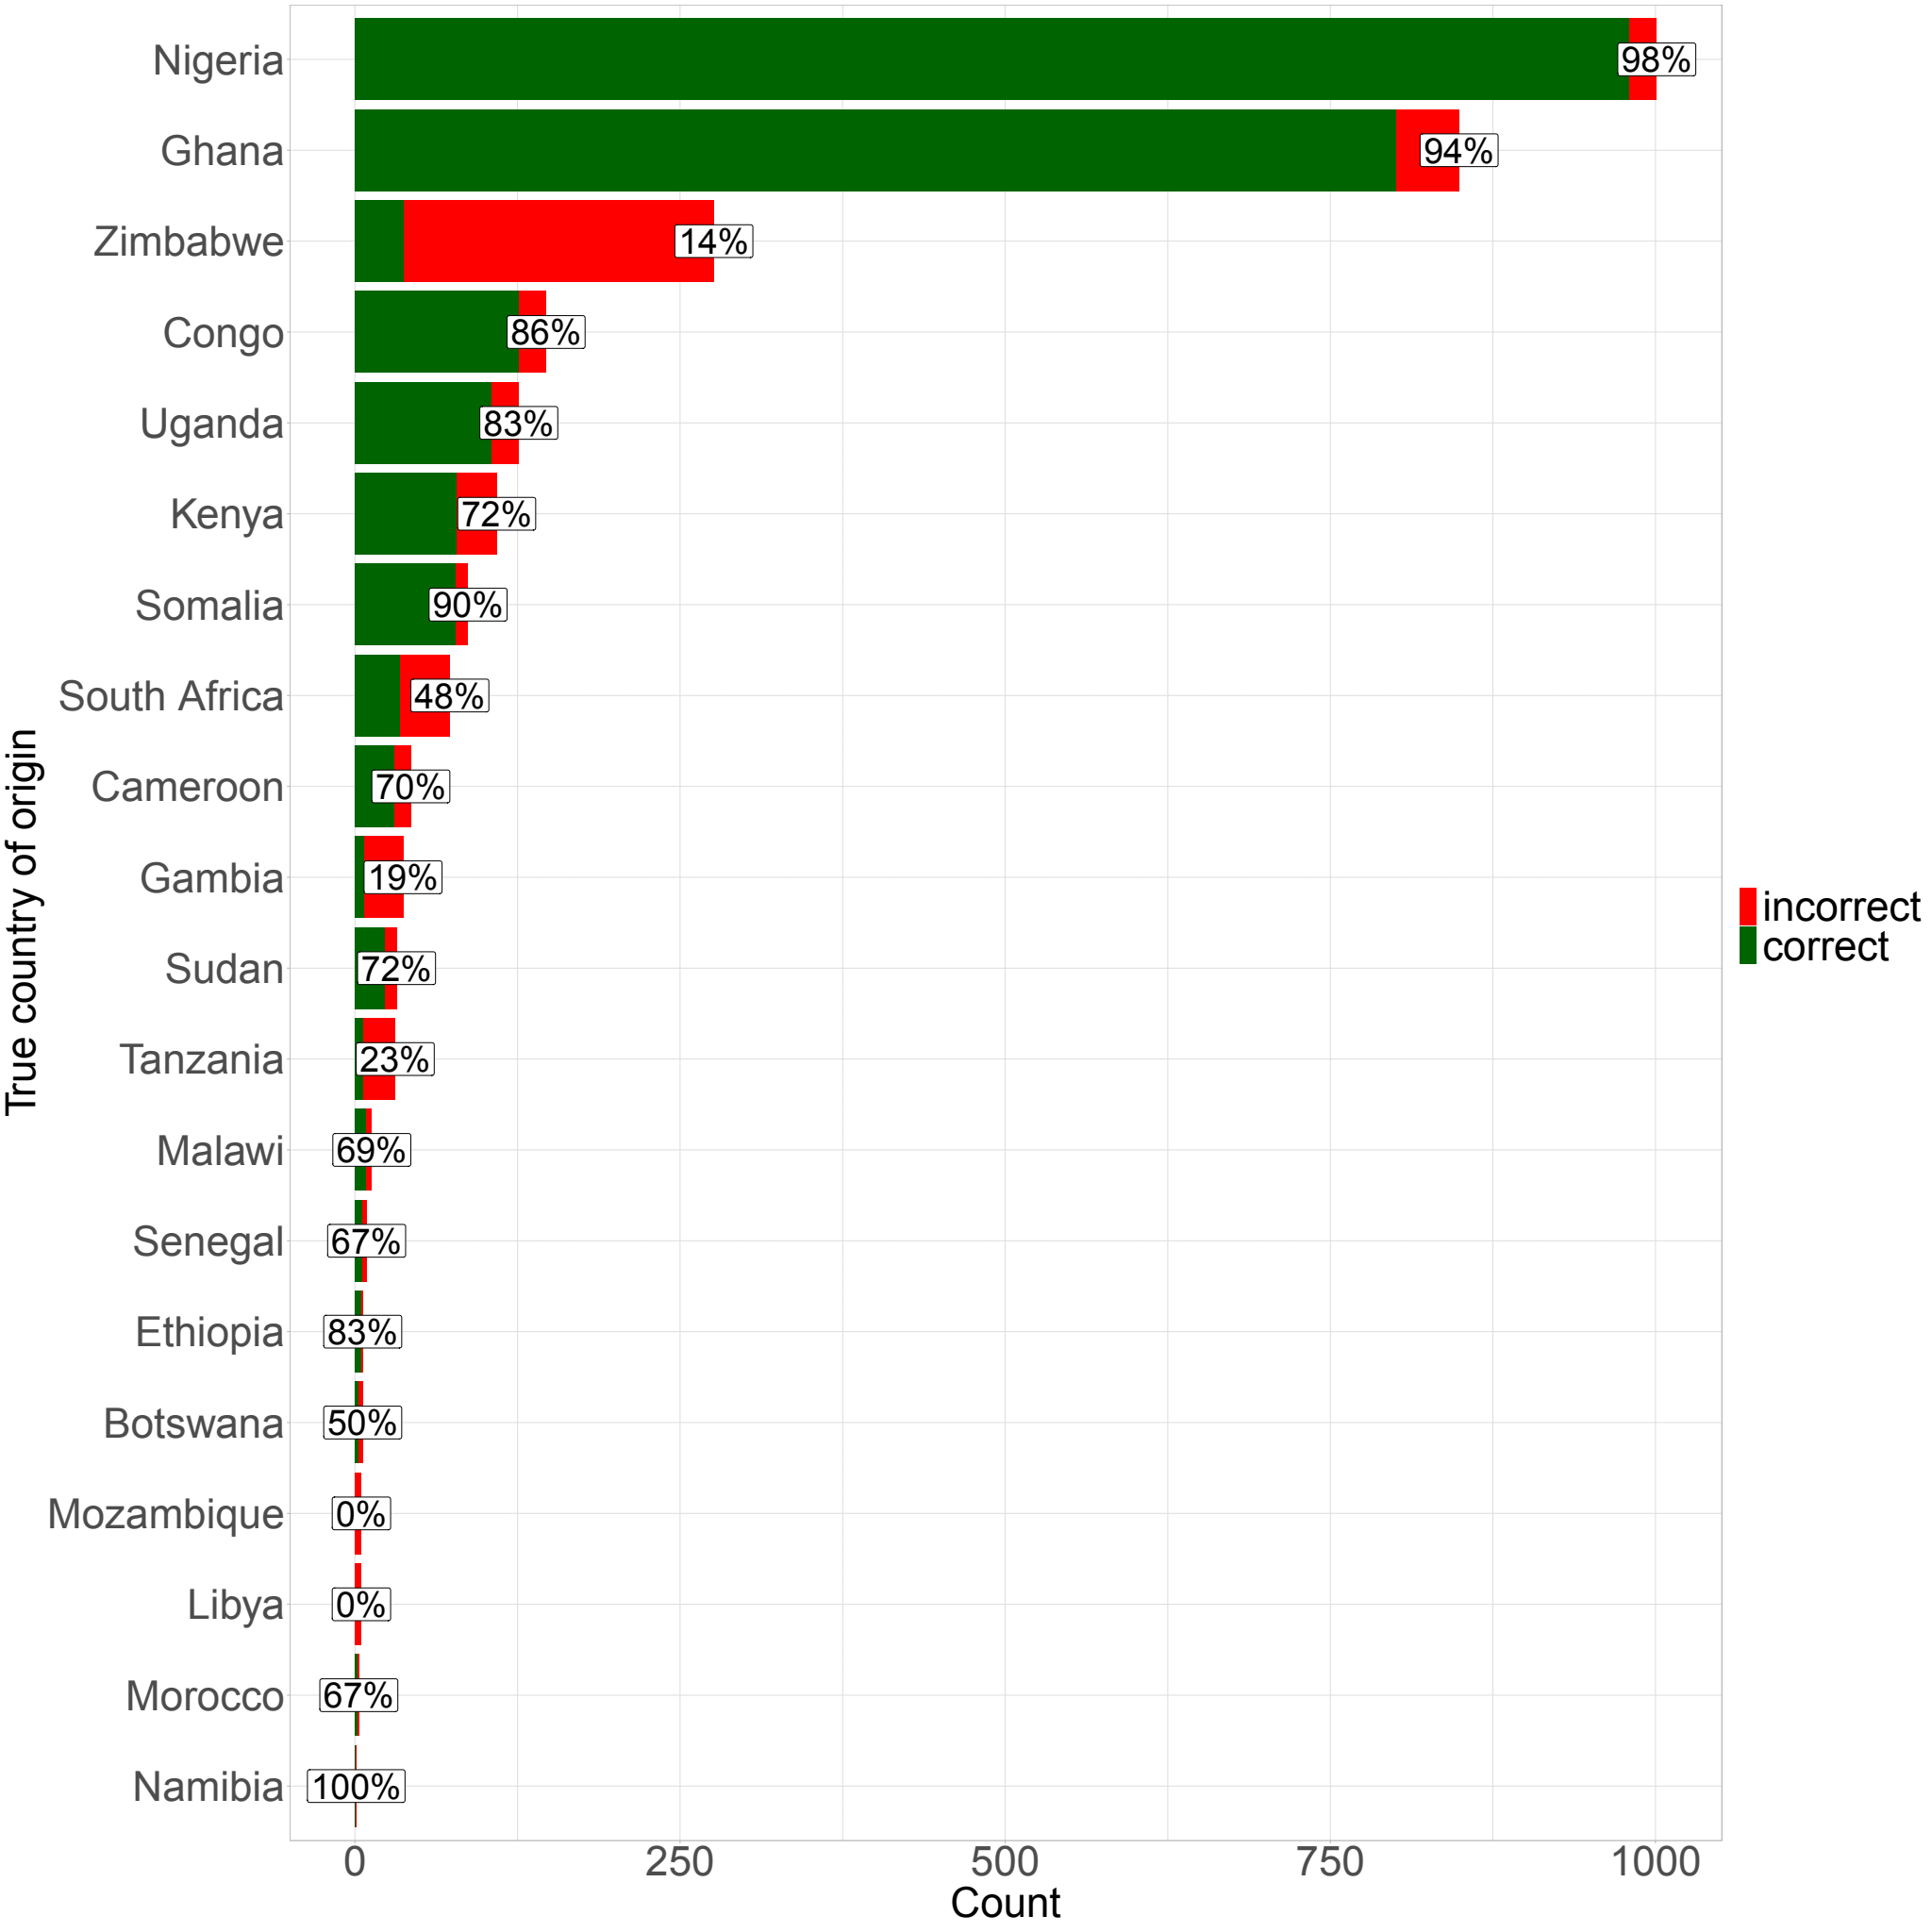
\includegraphics[width=1.0\textwidth]{../images/chapter3/country_of_origin_allInds.png}
    \caption{Correspondence of true birth country with estimated birth country. Each bar corresponds to a true birth country, with the length of the bar corresponding to the total number of people in our dataset born in that country. The green section corresponds to the total number of individuas where the birth country was correctly guessed and the red section to those who were incorrectly guessed. Percentage labels give percentage correct for that country.}
    \label{fig:country_of_origin_allInds}
\end{figure}

The overall accuracy at predicting birth location was 81.63\%, suggesting there was substantial information within the coancestry matrix. For the countries where there was a large number of reference populations, such as Ghana and Nigeria, the prediction accuracy was high. For certain countries, the prediction accuracy was much lower. For example, Tanzania was only represented by a single reference population. Zimbabwe...

\subsection{Imputation bias}

The imputed dataset consisted of 535,544 SNPs in total, 87.7\% of which were imputed. Having a high percentage of imputed SNPs may bias downstream analyses. 

For example, consider two UK Biobank individuals who have a large percentage of African ancestry. One of the individuals has ancestry relating to a particular Nigerian ethnic group and the other to a closely related, but different Nigerian ethnic group. We are interested in being able to determine the fine-scale differences in ancestry between these individuals. This relies on the existence of variants in each individual which are specific to that population.

Imputation relies on identifying reference haplotypes which are closest to the target haplotypes. However, neither of the ethnic groups that the individuals derive ancestry from are present in the imputation reference panel. Therefore, we would expect that the missing variants would be imputed from the populations in the reference panel which are most closely related to our target samples. In the case of the Haplotype Reference Consortium, the closest reference population to our two target samples may be the Yoruba. If missing are preferentially imputed from Yoruban individuals, then we would expect segments of the target samples to appear to me more 'Yoruba-like' than otherwise. Correspondingly, when painted using a reference panel which includes, but is not exclusive to, those populations found in the imputation reference panel, we would expect the populations found in the imputation reference panel to donate more.

Comparing the imputed and non-imputed coancestry matrices revealed biases consistent with the above expectation. If the coancestry matrix columns are combined into populations, then the sum of each column gives the total length of genome that population contributes to all recipient individuals in the dataset. Therefore, comparing the column sums between the imputed and non-imputed matrices informs us about which populations contribute more under in the imputed dataset than the non-imputed dataset. 

 \begin{figure}[htp]
    \centering
    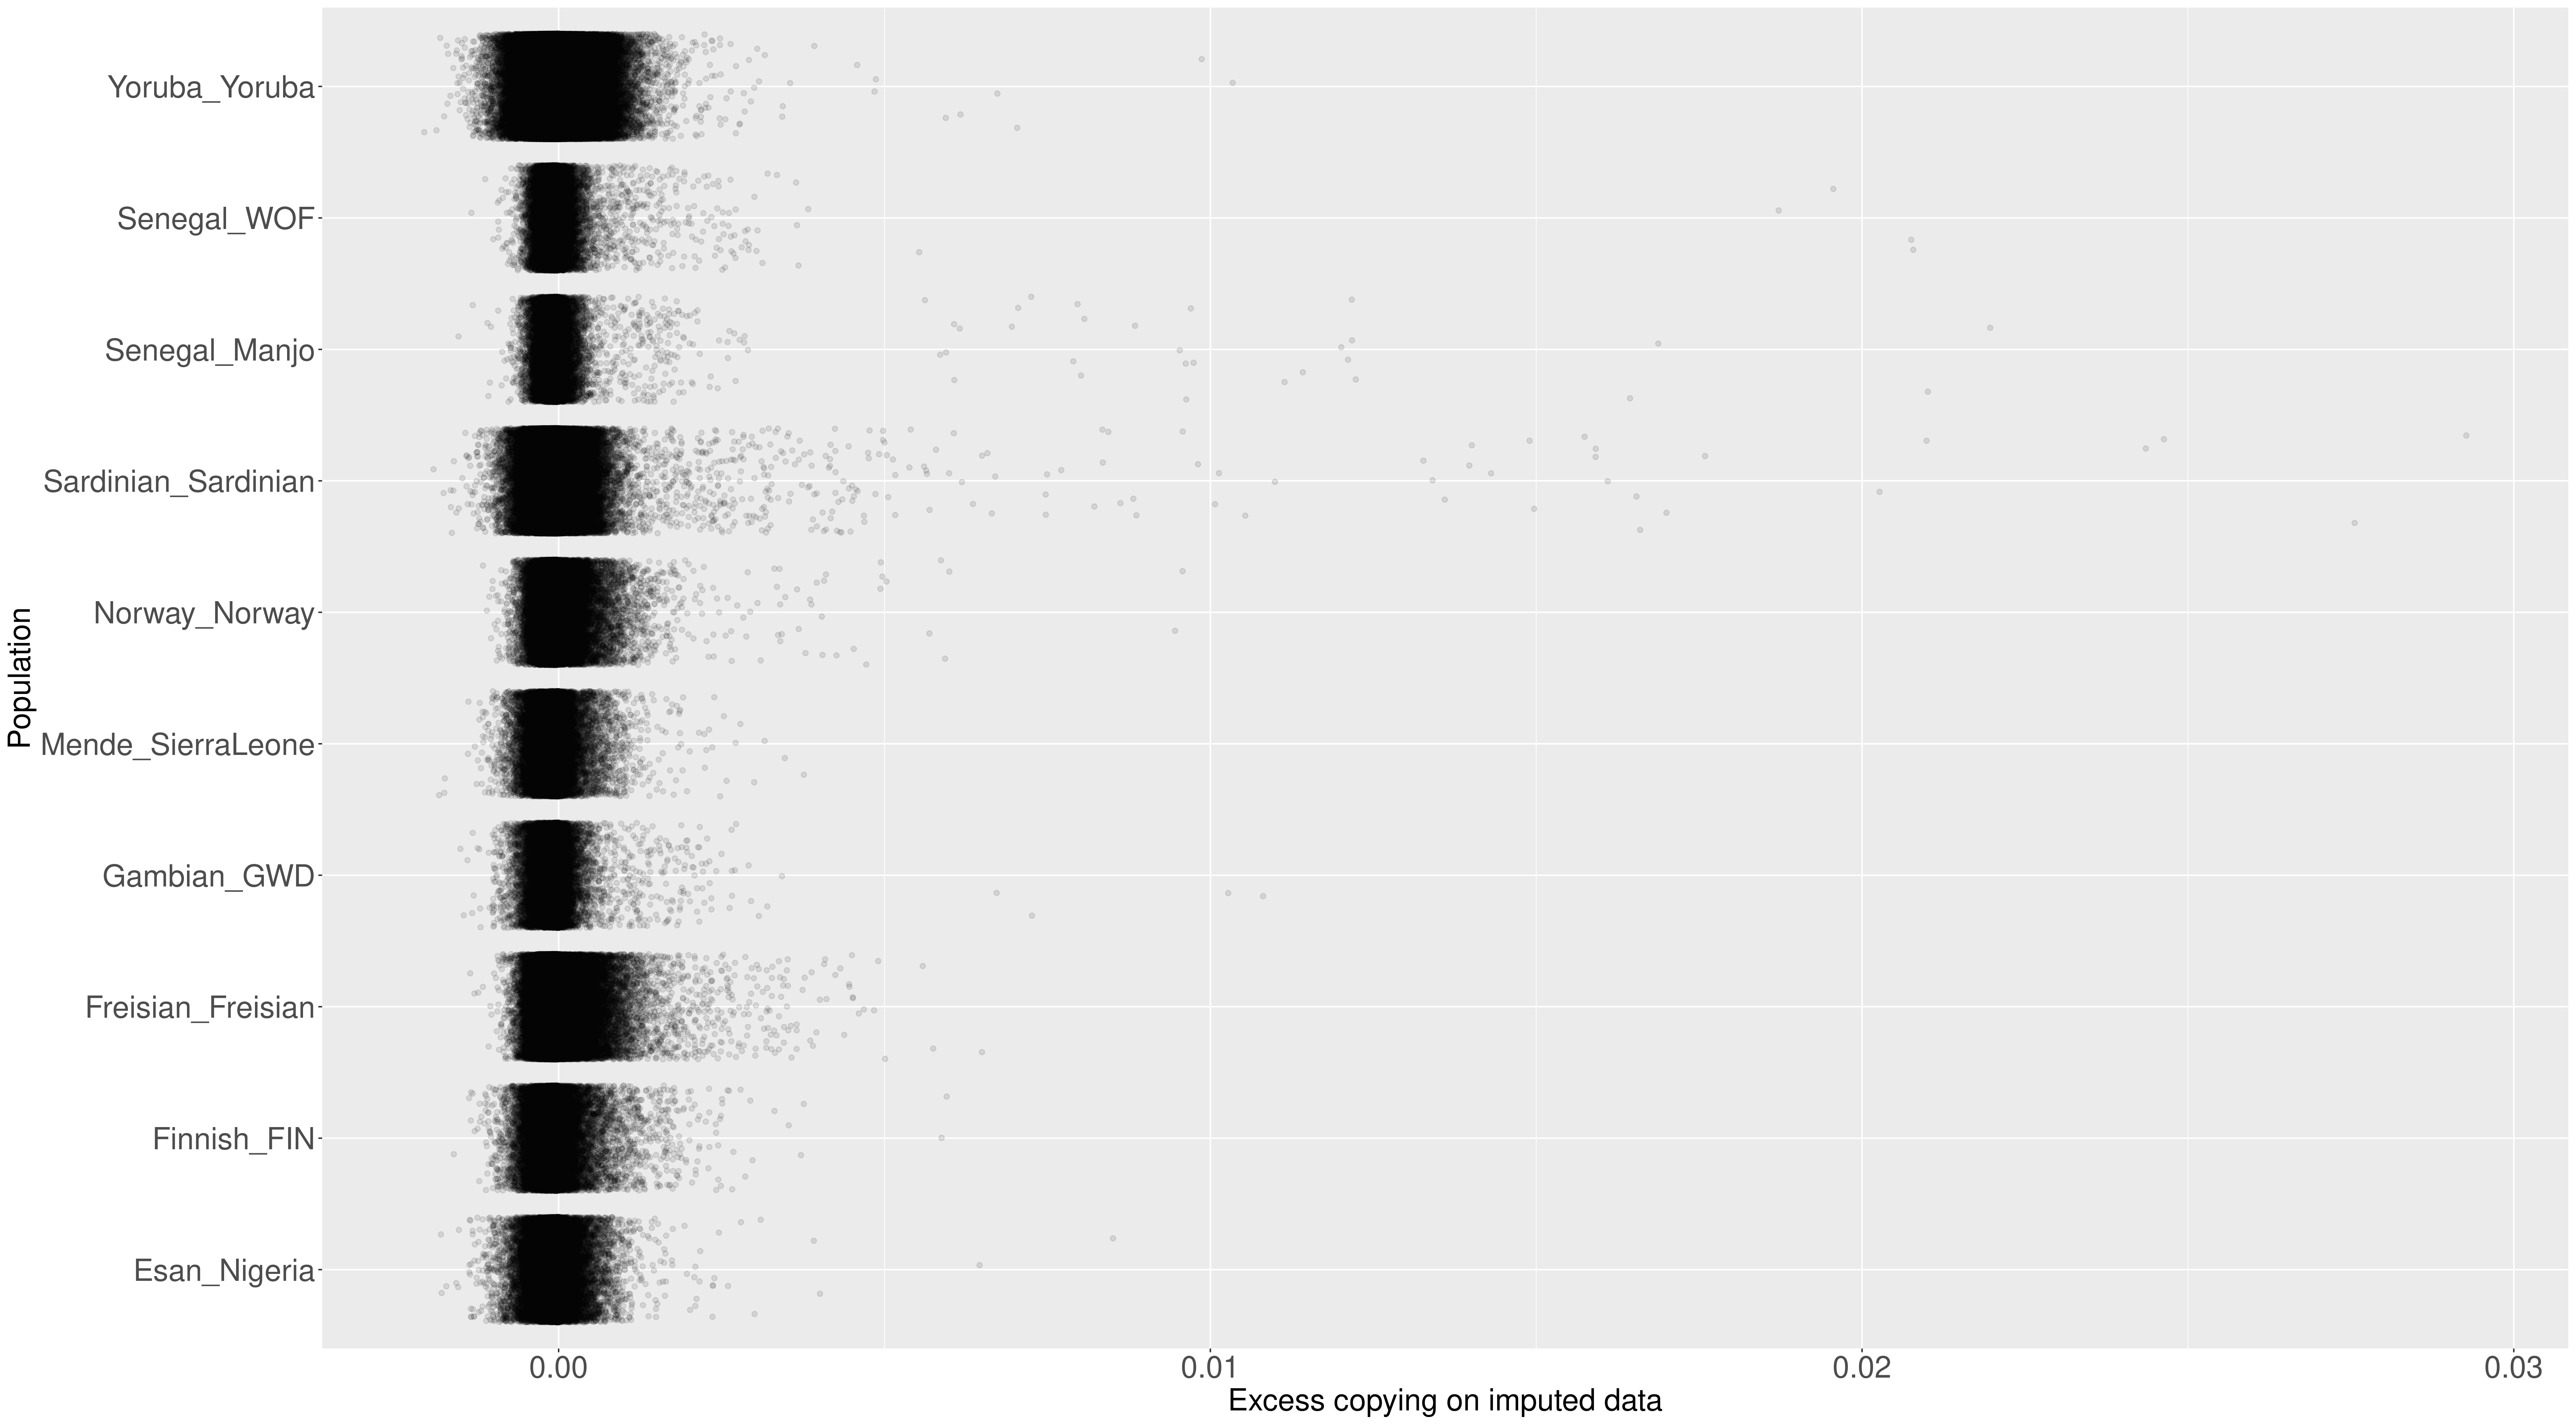
\includegraphics[width=1.0\textwidth]{../images/chapter3/imputed_excess_copying_pops.png}
    \caption{The top 10 Human Origins populations which donate more haplotypes under when data is imputed compared to non-imputed. Each point corresponds to the difference between the amount an individual from that donor population donated using imputed and non-imputed data, with positive values corresponding to more copying when the is imputed.}
    \label{fig:imputed_excess_copying_pops}
\end{figure}

Of the 568 populations tested, 6 were present in the 1000 genomes reference panel. 

Considering the SOURCEFIND results shows strong evidence that imputation alters the inferred ancestry proportions of the Human Origins individuals. If we take each target population and assign the surrogate with the largest ancestry proportion as the 'best surrogate', then only 30\% (144/478) of the best surrogates match between the imputed and non-imputed datasets. 









